\section{方差结构}
\label{sec:variance}

本节在 H1--H4 下比较两个估计目标的方差。目标Ⅰ的方差随规模趋于零，目标Ⅱ的方差有一个由环境决定的底板；两者之间的过渡由交叉点 $\mx$ 刻画。

\subsection{当期再生数}
\label{sec:variance-current}

先看目标Ⅰ。此时 $R_t$ 视为固定参数，估计量的性质由式~\eqref{eq:report-dist} 直接决定。

\begin{proposition}[当期再生数的有效估计]
\label{prop:current}
在 H1--H3 下，给定 $n$ 与 $R_t>0$，估计量 $\widehat R_t=C_t/(\rho n)$ 满足：
\begin{enumerate}[label=(\roman*)]
  \item $\widehat R_t$ 是 $R_t$ 的极大似然估计；当 $C_t=0$ 时，似然在边界 $R_t=0$ 处取最大值；
  \item $\widehat R_t$ 无偏，方差为 $\Var(\widehat R_t\mid n,R_t)=R_t/(\rho n)+R_t^2/(kn)$；
  \item 对任意 $n$，该方差都等于 Cramér--Rao 下界 $1/\mathcal I(R_t)$，其中 $\mathcal I(R_t)=n/(R_t/\rho+{R_t}^2/k)$；
  \item $\widehat R_t$ 是 $R_t$ 的一致最小方差无偏估计。
\end{enumerate}
\end{proposition}

结论 (iii) 不是渐近结果。得分函数恰好可以写成 $\mathcal I(R_t)(\widehat R_t-R_t)$ 的形式，所以下界在每个有限 $n$ 处都能取到。结论 (iv) 来自单参数指数族中 $C_t$ 的完备充分性，需要 $k$ 已知\citep{lehmann1998point, casella2002statistical}。方差由两部分组成，与式~\eqref{eq:relvar} 的两项一一对应，$R_t/(\rho n)$ 来自报告抽样，$R_t^2/(kn)$ 来自超传播。两部分都按 $1/n$ 衰减，规模越大，当期再生数估得越准，没有底板。

我们用蒙特卡洛模拟核对了命题~\ref{prop:current}(iii)。在 $m$ 从 1 到 1000 的 10 个规模上各做 20,000 次模拟，方差与 CRLB 之比在 0.98--1.02，差异来自蒙特卡洛误差（图~\ref{fig:variance}a 中的圆点）。

\subsection{跨期平均与交叉点}
\label{sec:variance-crossover}

目标Ⅱ要估计的是 $\Rbar$。$R_t$ 现在是随机的，估计误差多出了环境波动这一项。

\begin{proposition}[跨期平均水平的方差]
\label{prop:average}
在 H1--H4 下，$\widehat R_t=C_t/(\rho n)$ 是 $\Rbar$ 的无偏估计，其方差为
\begin{equation}
  V(m)=\Var(\widehat R_t\mid n)=v_R+\frac{\Rbar}{\rho n}+\frac{\Rbar^2+v_R}{kn}
  =v_R+\frac{A}{m},\qquad A=\Rbar+\frac{\rho(\Rbar^2+v_R)}{k}.
  \label{eq:var-average}
\end{equation}
定义交叉点 $\mx=A/v_R$，则：
\begin{enumerate}[label=(\roman*)]
  \item $m\to\infty$ 时 $V(m)\to v_R$；
  \item 规模项在总方差中的份额为 $1/(1+m/\mx)$，在 $m=\mx$ 处两项各占一半；
  \item 规模从 $m$ 翻倍到 $2m$，方差下降的比例为 $1/[2(1+m/\mx)]$；
  \item $V(m)$ 严格递减且严格凸，对 $m$ 的弹性为 $-\mx/(m+\mx)$，在 $m=\mx$ 处等于 $-1/2$。
\end{enumerate}
\end{proposition}

式~\eqref{eq:var-average} 由全方差公式得到。条件方差的期望给出 $A/m$，条件均值 $R_t$ 的方差给出 $v_R$。$A$ 中的二次项为 $\Rbar^2+v_R$，因为超传播项 $R_t^2/(kn)$ 要对 $R_t$ 取期望，而 $\E(R_t^2)=\Rbar^2+v_R$。

交叉点的含义要说清楚。$V(m)$ 处处凸，二阶导数为 $2A/m^3>0$，曲线上没有“转折”，所以 $\mx$ 不是收益突然消失的位置。它的作用是给规模提供一把尺子。规模低于 $\mx$ 时，误差主要来自病例太少，扩大规模收效明显；规模高于 $\mx$ 时，误差主要来自环境波动，翻倍的收益迅速变小。

图~\ref{fig:variance} 用一组示意参数画出这一结构，取 $\Rbar=1.15$，$v_R=0.04$，$k=0.35$，$\rho=0.25$。此时 $A=2.1232$，$\mx=53.1$。规模为 10、53.1 和 200 时，翻倍降幅依次为 42.1\%、25.0\% 和 10.5\%。目标Ⅱ的模拟方差与式~\eqref{eq:var-average} 之比同样落在 0.98--1.02。

\begin{figure}[!tbp]
  \centering
  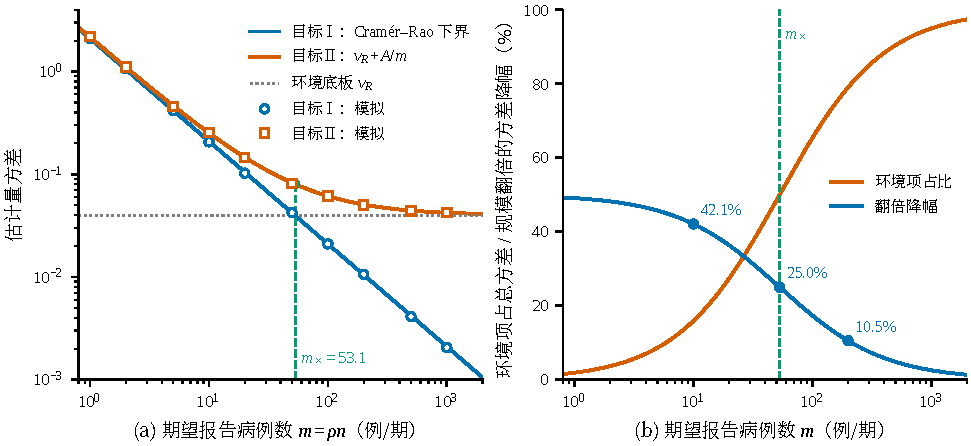
\includegraphics[width=\textwidth]{figures/fig_02_fig02_variance_theory.pdf}
  \caption{两个估计目标的方差结构。参数为 $\overline{R}=1.15$，$v_R=0.04$，$k=0.35$，$\rho=0.25$，对应 $A=2.1232$，$m_\times=53.1$。(a) 目标Ⅰ的方差（即 Cramér--Rao 下界，取 $R_t=\overline{R}$）与目标Ⅱ的方差 $v_R+A/m$ 随规模的变化，空心点为每个规模 20,000 次模拟的方差，虚线标出交叉点。(b) 环境项在目标Ⅱ总方差中的占比，以及规模翻倍带来的方差降幅；三个标注点对应 $m=10$、$m_\times$ 与 $200$。}
  \label{fig:variance}
\end{figure}

底板 $v_R$ 在单一环境内无法通过扩大规模消除，但可以通过汇总多个环境来压低。设 $J$ 个辖区的环境方差同为 $v_R$，两两相关系数的平均值为 $\bar c$。等权汇总后，环境项变为
\begin{equation}
  v_R\,\bar c+\frac{v_R(1-\bar c)}{J}.
  \label{eq:pooling}
\end{equation}
各辖区的扰动不完全同步时（$\bar c<1$），汇总能降低底板；完全同步时汇总无效。第~\ref{sec:empirical-robust}~节会用全国加总序列估计 $\bar c$。

\subsection{报告率与覆盖面}
\label{sec:variance-reporting}

$m=\rho n$ 可以通过两条途径扩大，即提高报告率 $\rho$，或扩大覆盖的人群使 $n$ 增大。式~\eqref{eq:var-average} 表明两者的作用并不相同。

\begin{proposition}[报告率与覆盖面的不对称]
\label{prop:reporting}
在 H1--H4 下：
\begin{enumerate}[label=(\roman*)]
  \item 固定 $n$ 令 $\rho\to1$，$V\to v_R+\Rbar/n+(\Rbar^2+v_R)/(kn)$，极限严格大于 $v_R$；
  \item 固定 $\rho$ 令 $n\to\infty$，$V\to v_R$；
  \item 报告项可以拆为 $\Rbar/(\rho n)=\Rbar/n+(1-\rho)\Rbar/(\rho n)$，第二部分是漏报带来的额外方差；
  \item 把 $n$ 与 $\rho$ 各提高相同的小比例，前者带来的方差下降是后者的 $A/\Rbar=1+\rho(\Rbar^2+v_R)/(k\Rbar)$ 倍。
\end{enumerate}
\end{proposition}

命题~\ref{prop:reporting} 说明，提高报告率与扩大覆盖的作用不对称。即使报告完全，超传播项仍然存在，只有扩大覆盖才能把方差压到 $v_R$。不过，两者的差距取决于 $\rho$ 的大小。在图~\ref{fig:variance} 的参数下，$A/\Rbar=1.85$，扩大覆盖的效果接近提高报告率的两倍。在流感住院监测中，住院占感染的比例约为 0.0056--0.021\citep{zhou2012hospitalizations, tokars2018seasonal}。取第~\ref{sec:empirical-early}~节的情景参数，这一倍数只有 1.02--1.18。也就是说，对住院数据而言，两条途径的效果几乎相同，选择哪一条主要看成本。
